\documentclass[12pt]{ctexart}
\usepackage{amssymb,amsmath,makecell}
\usepackage{hyperref}
\usepackage{booktabs}
\usepackage[nofonts]{ctexcap}
\usepackage{setspace}
\usepackage{graphicx}
\usepackage{fix-cm}
\usepackage{enumerate}
\usepackage{float}
\usepackage{graphicx}
\usepackage{fancybox}
\usepackage{longtable}
\usepackage{multirow}
\usepackage{minted}
\usepackage{pdfpages}
\usepackage[ruled,vlined]{algorithm2e}
\usepackage[normalem]{ulem}
\useunder{\uline}{\ul}{}
\usepackage{tikz}
\usetikzlibrary{automata, positioning, arrows.meta, arrows}

\usepackage[bjydu]{cnlogo}
\definecolor{bjydu}{RGB}{0,51,153}

\newmintinline{cpp}{breaklines,breakanywhere}
\newminted{cpp}{breakanywhere,breaklines,linenos,frame=single}

\newcommand{\bigsize}{\fontsize{25pt}{20pt}\selectfont}
% \setCJKmainfont[BoldFont=STFangsong]{STFangsong}
% Page length commands go here in the preamble
\setlength{\oddsidemargin}{-0.25in} % Left margin of 1 in + 0 in = 1 in
\setlength{\textwidth}{7in}   % Right margin of 8.5 in - 1 in - 6.5 in = 1 in
\setlength{\topmargin}{-.75in}  % Top margin of 2 in -0.75 in = 1 in
\setlength{\textheight}{9.2in}  % Lower margin of 11 in - 9 in - 1 in = 1 in

\newtheorem{theorem}{Theorem}
\newtheorem{definition}{Definition}
\newcommand{\ulinebox}[1]{\underline{\makebox[5cm][c]{#1}}}

\renewcommand{\baselinestretch}{1.5} % 1.5 denotes double spacing. Changing it will change the spacing

\hypersetup{colorlinks=true,linkcolor=black,filecolor=magenta,urlcolor=cyan}
\setlength{\parindent}{0in}

\begin{document}
% \CTEXsetup[format={\Large\bfseries}]{section}
% \CTEXsetup[number={\chinese{section}}]{section}
\begin{titlepage}
    \center
    
\includegraphics[width=3.5in]{images/buptname.eps}

    \begin{spacing}{5}
        {\bigsize \textbf{设计报告}}
    \end{spacing}

    % \includegraphics[width=2.3in]{images/buptseal.eps}
    \bjydulogo[bjydu][1.8]

    \begin{spacing}{1}
        \vspace{1.5cm}
        \Large \begin{tabular}{@{}l@{}}
            课程名称: \ulinebox{算法设计与分析} \\
            实验名称: \ulinebox{分治法的应用} \\
            学\qquad 院: \ulinebox{计算机学院} \\
            班\qquad 级: \ulinebox{2022211312} \\
            学\qquad 号: \ulinebox{2022211404} \\
            姓\qquad 名: \ulinebox{唐梓楠}
        \end{tabular}
        \vspace{2.5cm}
    \end{spacing}

    {\small\em \today }
\end{titlepage}


\newpage

\tableofcontents

\newpage
\allowdisplaybreaks
\section{一般原理}

\subsection{定义}

\begin{definition}[分治 Divide and Conquer]
    字面上的解释是 ``分而治之'',就是把一个复杂的问题分成两个或更多的相同或相似的子问题,直到最后子问题可以简单的直接求解,原问题的解即子问题的解的合并。
\end{definition}

\subsection{过程}

分治算法的核心思想就是 ``分而治之''。

大概的流程可以分为三步:\textbf{分解 $\to$ 解决(触底) $\to$ 合并(回溯)}。\begin{enumerate}
    \item 分解原问题为结构相同的子问题。
    \item 分解到某个容易求解的边界之后,进行递归求解。
    \item 将子问题的解合并成原问题的解。
\end{enumerate}
分治法能解决的问题一般有如下特征:\begin{itemize}
    \item 该问题的规模缩小到一定的程度就可以容易地解决。
    \item 该问题可以分解为若干个规模较小的相同问题,即该问题具有\textbf{最优子结构性质}。
    \item 利用该问题分解出的子问题的解可以合并为该问题的解。
    \item 该问题所分解出的各个子问题是相互独立的,即子问题之间不包含公共的子问题。
\end{itemize}

如果各子问题是不独立的,则分治法要重复地解公共的子问题,也就做了许多不必要的工作。此时虽然也可用分治法,但一般用\textbf{动态规划}较好。

在用分治法设计算法时,最好使子问题的规模大致相同:即将一个问题分成大小相等的 $k$ 个子问题的处理方法是行之有效的。这种使子问题规模大致相等的做法是出自一种\textbf{平衡(balancing)子问题}的思想,它几乎总是比子问题规模不等的做法要好。

\subsection{递归与分治的区别}

递归是一种编程技巧,一种解决问题的思维方式;分治算法很大程度上是基于递归的,解决更具体问题的算法思想。

\section{问题}

给定一个有 $n$ 个数的无序的数组,查找其中排序好后的第 $k$ 大的元素(排序从1开始)。

比较不同规模下 $n=1000,100000,1000000$ 到 10000000,且 $k$ 取在有序后的头部、中间和尾部时(比如,间隔为 $n/8$ 的方式)各自的时间复杂度,比较相关的差异,画出曲线图。

\section{算法设计}

\subsection{随机选择}

\subsubsection{基本流程}

\begin{algorithm}[htbp]
    \label{alg:quickSelect}
    \SetAlgoLined
    \SetKwInput{KwIn}{输入}
    \SetKwInput{KwOut}{输出}
    \KwIn{数组 $nums$, 左边界 $left$, 右边界 $right$, 第 $k$ 大的元素位置 $k$, 随机数生成器 $gen$}
    \KwOut{第 $k$ 大的元素}
    
    \If{$left == right$}{
        \Return $nums[left]$\;
    }
    
    % 随机选择枢轴
    $pivotIndex \leftarrow$ 随机整数生成于 $[left, right]$ \;
    $pivot \leftarrow nums[pivotIndex]$\;
    
    % 将枢轴移到末尾
    交换 $nums[pivotIndex]$ 和 $nums[right]$\;
    
    % 分区操作
    $storeIndex \leftarrow left$\;
    \For{$i \leftarrow left$ \textbf{to} $right - 1$}{
        \If{$nums[i] > pivot$}{ % 查找第 k 大,因此使用 > 符号
            交换 $nums[i]$ 和 $nums[storeIndex]$\;
            $storeIndex \leftarrow storeIndex + 1$\;
        }
    }
    
    % 将枢轴放到正确的位置
    交换 $nums[storeIndex]$ 和 $nums[right]$\;
    
    % 计算枢轴位置相对于第 k 大的位置
    $count \leftarrow storeIndex - left + 1$\;
    \If{$count == k$}{
        \Return $nums[storeIndex]$\;
    }
    \ElseIf{$k < count$}{
        \Return \textbf{quickSelect}($nums$, $left$, $storeIndex - 1$, $k$, $gen$)\;
    }
    \Else{
        \Return \textbf{quickSelect}($nums$, $storeIndex + 1$, $right$, $k - count$, $gen$)\;
    }
    
    \caption{基于随机选择方式的分治法查找第 $k$ 大元素}
    \end{algorithm}    
    \begin{description}
        \item[基线情况] 如果当前查找范围内只有一个元素,直接返回该元素。
        \item[随机选择枢轴] 在当前范围内随机选择一个枢轴元素,并将其移动到数组的末尾。
        \item[分区操作] 将所有大于枢轴的元素移动到左侧,记录分割点 \texttt{storeIndex}。
        \item[递归查找] \begin{itemize}
            \item 如果枢轴的位置正好是第 $k$ 大的位置,返回枢轴元素。
            \item 如果第 $k$ 大的元素在左侧子数组中,递归查找左侧。
            \item 否则,在右侧子数组中继续查找,并调整 $k$ 的值。
        \end{itemize}
    \end{description}
    算法伪代码如算法~\autoref{alg:quickSelect} 所示。
\subsubsection{复杂度分析}

\textbf{最好情况}:每次选择的枢轴将数组\textbf{近乎等分},即每次分割后,左右子数组的大小均为 $\frac{n}{2} $。	例如,枢轴总是将数组分为一个大小为 $\frac{n}{2}$ 的子数组和一个大小为 $\frac{n}{2} - 1$ 的子数组。

由于每次分区需要遍历当前数组范围,时间为 $O(n)$,每次将问题规模减半,因此递归深度为 $O(\log n)$。每层递归都进行一次 $O(n)$ 的操作,递归深度为 $O(\log n)$。

设 $T(n)$ 为在大小为 $n$ 的数组上执行 \texttt{quickSelect} 的时间。根据最好情况,递归关系为:
\[T(n) = T\left(\frac{n}{2}\right) + O(n)\]

我们可以使用递归树的方法来解这个递归关系。\begin{itemize}
    \item 第 0 层:一次 $O(n)$ 的操作。
    \item 第 1 层:一次 $O(\frac{n}{2})$ 的操作。
    \item 第 2 层:一次 $O(\frac{n}{4})$ 的操作。
    \item $\cdots$
    \item 第 $\log n$ 层:一次 $O(1)$ 的操作。
\end{itemize}

总时间为各层之和:\[T(n) = O(n) + O\left(\frac{n}{2}\right) + O\left(\frac{n}{4}\right) + \dots + O(1) = O(n) \left(1 + \frac{1}{2} + \frac{1}{4} + \dots \right) = O(n) \times 2 = O(n)\]

因此在最好情况下,\texttt{quickSelect} 的时间复杂度为 $O(n)$。

\textbf{最坏情况}:每次选择的枢轴是当前范围内的\textbf{最大}或\textbf{最小}元素,导致一侧子数组为空或仅含一个元素,另一侧子数组大小为 $n - 1$。例如,每次枢轴选择都将数组分为一个大小为 1 的子数组和一个大小为 $n - 1$ 的子数组。

每次分区需要遍历当前数组范围,时间为 $O(n)$,每次仅减去一个元素,因此递归深度为 $O(n)$,可以列出递归关系式为\[T(n) = T(n - 1) + O(n)\]

展开递归关系有 \begin{itemize}
    \item $T(n)=T(n-1)+cn$
    \item $T(n-1)=T(n-2)+c(n-1)$
    \item $\cdots$
    \item $T(2)=T(1)+2c$
    \item $T(1)=c$
\end{itemize}

将所有展开项相加:\[T(n) = c + 2c + 3c + \dots + nc = c \sum_{i=1}^{n} i = c \cdot \frac{n(n + 1)}{2} = O(n^2)\]

因此在最坏情况下,\texttt{quickSelect} 的时间复杂度为 $O(n^2)$。

\textbf{平均情况}:枢轴的选择是\textbf{随机的},导致数组在每次分区时,左右子数组的大小具有概率分布,通常接近均匀分布。例如,枢轴平均将数组分为大小约为 $\alpha n$ 和 $(1 - \alpha)n$ 的子数组,其中 $0 < \alpha < 1$。

为了分析平均情况,我们需要计算 \texttt{quickSelect} 的期望时间复杂度。由于枢轴是随机选择的,分区后左右子数组的大小是随机的。

设 $E(n)$ 为在大小为 $n$ 的数组上执行 \texttt{quickSelect} 的期望时间。分区操作需要 $O(n)$ 的时间,随后根据枢轴的位置,递归调用较小的一侧。因此递归关系为:\[E(n)=E(\text{数组大小}) + O(n)\]

具体地,设枢轴位置为第 $p$ 个元素(1-based),则有:
\begin{itemize}
    \item 如果 $p = k$,直接返回,时间为 $O(n)$。
	\item 如果 $p > k$,递归调用左侧子数组,大小为 $p - 1$。
	\item 如果 $p < k$,递归调用右侧子数组,大小为 $n - p$。
\end{itemize}

由于枢轴是随机选择的, $p$ 在 $[1, n]$ 上均匀分布。因此, $p$ 的概率分布为均匀分布。可以写为:
\[E(n)=\frac{1}{n}\sum_{p=1}^{n}\begin{cases}
    E(p-1)+O(n) & \text{if } p>k\\
    E(n-p)+O(n) & \text{if } p<k\\
    O(n) & p=k
\end{cases}\]

考虑到 \texttt{quickSelect} 只会递归调用一侧,且在每次递归时只处理一个子数组,因此:
\[E(n)=O(n)+\frac{1}{n}\sum_{p=1}^{n}[E(\max(p-1,n-p))]\]

采用\textbf{数学归纳法}进行证明,假设 \( E(m) \leq c m \) 对于所有 \( m < n \) 成立,则:\[
E(n) \leq c n + \frac{1}{n} \sum_{p=1}^{n} c \cdot \max(p - 1, n - p)
\]

考虑 \( \max(p - 1, n - p) \),这取决于 \( p \) 的位置。\begin{itemize}
    \item 对于 \( p \leq \frac{n}{2} \),有 \( \max(p - 1, n - p) = n - p \)。
    \item 对于 \( p > \frac{n}{2} \),有 \( \max(p - 1, n - p) = p - 1 \)。
\end{itemize}

因此:\[
\sum_{p=1}^{n} \max(p - 1, n - p) = \sum_{p=1}^{\lfloor n/2 \rfloor} (n - p) + \sum_{p=\lfloor n/2 \rfloor + 1}^{n} (p - 1)
\]

计算这两个和:\begin{enumerate}
    \item \textbf{前半部分}(\( p = 1 \) 到 \( p = \lfloor n/2 \rfloor \)):\[
    \sum_{p=1}^{\lfloor n/2 \rfloor} (n - p) = \lfloor n/2 \rfloor n - \sum_{p=1}^{\lfloor n/2 \rfloor} p = \lfloor n/2 \rfloor n - \frac{\lfloor n/2 \rfloor (\lfloor n/2 \rfloor + 1)}{2}
    \]
    
    近似为 \( \frac{n^2}{4} \)。
    
    \item \textbf{后半部分}(\( p = \lfloor n/2 \rfloor + 1 \) 到 \( p = n \)):\[
    \sum_{p=\lfloor n/2 \rfloor + 1}^{n} (p - 1) = \sum_{p=\lfloor n/2 \rfloor + 1}^{n} p - \sum_{p=\lfloor n/2 \rfloor + 1}^{n} 1 = \sum_{p=1}^{n} p - \sum_{p=1}^{\lfloor n/2 \rfloor} p - (n - \lfloor n/2 \rfloor)
    \]

    近似为 \( \frac{n^2}{4} \)。
\end{enumerate}

因此,整体和为 \( \sum_{p=1}^{n} \max(p - 1, n - p) \approx \frac{n^2}{2} \)。

将其代入递归关系:\[
E(n) \leq c n + \frac{1}{n} \cdot c \cdot \frac{n^2}{2} = c n + \frac{c n}{2} = \frac{3}{2} c n
\]

因此,可以选择 \( c \) 使得 \( \frac{3}{2} c \leq c' \)(例如 \( c' = 2c \)),则归纳假设成立。表明:\[
E(n) = O(n)
\]

因此在平均情况下,\texttt{quickSelect} 的时间复杂度为 \( O(n) \)。

尽管最坏情况下时间复杂度较高,但由于随机选择枢轴的策略,最坏情况发生的概率极低。因此,在实际应用中,\texttt{quickSelect} 通常表现出线性的时间复杂度。

\textbf{空间复杂度分析}:对于空间复杂度,我们主要关注算法在执行过程中所需的额外内存空间,因此输入数据存储不计入空间复杂度。算法操作的是输入数组 \texttt{nums},但由于操作是原地进行(即在原数组上进行元素交换),因此不需要额外的数组存储空间。由于 \texttt{quickSelect} 是一个递归算法,且由于传递参数时,传递的是数组的引用,因此递归调用的栈空间不会产生对原数组的拷贝,但是算法中使用了少量的辅助变量(如 \texttt{pivotIndex}、\texttt{pivot}、\texttt{storeIndex} 等),这些变量的空间需求与输入规模无关,可以视为常数,由于会有常数的栈空间开销,空间递归深度直接影响算法的空间复杂度。

由前面的分析我们可以知道递归深度,因此很容易可以得出,平均情况下 \texttt{quickSelect} 的空间复杂度为 \( O(\log n) \),最坏情况下的空间复杂度为 \( O(n) \)。

\subsection{确定的线性时间选择}

\subsubsection{基本流程}

\begin{algorithm}[htbp]
    \label{alg:deterministicSelect}
    \SetAlgoLined
    \DontPrintSemicolon
    \SetKwInOut{Input}{输入}
    \SetKwInOut{Output}{输出}
    
    \Input{数组 $nums$, 左边界 $left$, 右边界 $right$, 第 $k$ 大的元素位置 $k$}
    \Output{第 $k$ 大的元素}
    
    \If{$right - left + 1 \leq 5$}{
        \Return \textbf{findMedian}($nums$, $left$, $right$)\;
    }
    
    % 将数组分成每组最多5个元素,找到每组的中位数
    $medians \leftarrow \emptyset$\;
    \For{$i \leftarrow left$ \textbf{to} $right$ \textbf{step} 5}{
        $sub\_right \leftarrow \min(i + 4, right)$\;
        $median \leftarrow$ \textbf{findMedian}($nums$, $i$, $sub\_right$)\;
        $medians.\text{append}(median)$\;
    }
    
    % 递归地找到中位数的中位数
    $medianOfMedians \leftarrow$ \textbf{deterministicSelect}($medians$, $0$, $medians.\text{size()} - 1$, $\lceil \frac{medians.\text{size()}}{2} \rceil$)\;
    
    % 找到中位数的索引
    $pivotIndex \leftarrow$ \textbf{findIndex}($nums$, $left$, $right$, $medianOfMedians$)\;
    
    % 将枢轴移到末尾
    \textbf{swap}($nums[pivotIndex]$, $nums[right]$)\;
    
    % 分区操作
    $storeIndex \leftarrow left$\;
    \For{$i \leftarrow left$ \textbf{to} $right - 1$}{
        \If{$nums[i] > medianOfMedians$}{ % 查找第 $k$ 大,因此使用 > 符号
            \textbf{swap}($nums[i]$, $nums[storeIndex]$)\;
            $storeIndex \leftarrow storeIndex + 1$\;
        }
    }
    
    % 将枢轴放到正确的位置
    \textbf{swap}($nums[storeIndex]$, $nums[right]$)\;
    
    % 计算枢轴位置相对于第 $k$ 大的位置
    $count \leftarrow storeIndex - left + 1$\;
    \If{$count == k$}{
        \Return $nums[storeIndex]$\;
    }
    \ElseIf{$k < count$}{
        \Return \textbf{deterministicSelect}($nums$, $left$, $storeIndex - 1$, $k$)\;
    }
    \Else{
        \Return \textbf{deterministicSelect}($nums$, $storeIndex + 1$, $right$, $k - count$)\;
    }
    
    \caption{基于确定性选择的分治法查找第 $k$ 大元素}
    \end{algorithm}
    \begin{algorithm}[htbp]
        \label{alg:findMedian}
        \SetAlgoLined
        \DontPrintSemicolon
        \SetKwInOut{Input}{输入}
        \SetKwInOut{Output}{输出}
        
        \Input{数组 $nums$, 左边界 $left$, 右边界 $right$}
        \Output{中位数元素}
        % 对子数组 [left, right] 进行排序
        \textbf{Sort}($nums[left \dots right]$)\;
        
        % 计算中位数的索引
        $medianIndex \leftarrow left + \left\lfloor \frac{right - left}{2} \right\rfloor$\;
        
        % 返回中位数
        \Return $nums[medianIndex]$\;
        
        \caption{查找子数组的中位数}
    \end{algorithm}

    \begin{description}
        \item[基线情况] 如果当前查找范围内元素数量不超过5,直接找到并返回中位数。
        \item[分组与中位数收集] 将数组分成每组最多5个元素,分别找到每组的中位数,并将这些中位数存入 \texttt{medians} 数组。
        \item[中位数的中位数]: 递归调用 \texttt{deterministicSelect} 函数,找到 \texttt{medians} 数组的中位数,即 ``中位数的中位数''。
        \item[分区操作] 使用 ``中位数的中位数'' 作为枢轴,对数组进行分区,使得所有大于枢轴的元素位于左侧,记录分割点 \texttt{storeIndex}。
        \item[递归查找] \begin{itemize}
            \item 如果枢轴的位置正好是第 $k$ 大的位置,返回该元素。
            \item 如果第 $k$ 大的元素在左侧子数组中,递归查找左侧子数组。
            \item 否则,在右侧子数组中继续查找,并调整 $k$ 的值。
        \end{itemize}
    \end{description}

    算法伪代码如算法~\autoref{alg:deterministicSelect} 所示,其调用的寻找中位数的子算法如算法~\autoref{alg:findMedian} 所示。
\subsubsection{复杂度分析}

\textbf{最好情况}:每次选择的枢轴 ``中位数的中位数'' 能够将数组近乎均匀地分割为两部分,即每次分割后,左右子数组的大小大致相等(接近 \( \frac{n}{2} \))。将数组分成大小不超过 5 的组,每组找到中位数需要 \( O(1) \) 时间(常数时间内完成排序和选择中位数)。总共 \( \frac{n}{5} \) 组,时间复杂度为 \( O(n) \)。在 \texttt{medians} 数组中找到中位数,需要递归调用 \texttt{deterministicSelect},子问题规模为 \( \frac{n}{5} \)。在分区操作时,需要对数组进行一次线性扫描和分区,时间复杂度为 \( O(n) \)。由于每次分割均匀,递归深度为 \( O(\log n) \)。

设 \( T(n) \) 为大小为 \( n \) 的数组上执行 \texttt{deterministicSelect} 的时间,最好情况下的递归关系为:\[
T(n) = T\left(\frac{n}{5}\right) + O(n)
\]
\begin{theorem}[主定理 Master Theorem]
    对于递推关系式\[
T(n) = a \cdot T\left(\frac{n}{b}\right) + f(n)
\]其中:\begin{itemize}
    \item \( a \geq 1 \):表示每次递归调用的子问题数量。
    \item \( b > 1 \):表示问题规模被分割的比例。
    \item \( f(n) \):表示在分治步骤中所花费的额外时间(例如,分割和合并的时间)。
\end{itemize}
主定理根据函数 \( f(n) \) 与 \( n^{\log_b a} \) 的关系,将递归关系分为以下三种情况,每种情况对应不同的渐近时间复杂度。\begin{enumerate}
    \item 多项式次的较小额外工作:如果存在常数 \( \varepsilon > 0 \) 使得:\[
    f(n) = O\left(n^{\log_b a - \varepsilon}\right)
    \]
    则递归关系的解为:\[
    T(n) = \Theta\left(n^{\log_b a}\right)
    \]
    在这种情况下,分治过程中额外的工作 \( f(n) \) 相对于递归调用的工作量 \( n^{\log_b a} \) 来说较小,因此总体时间复杂度主要由递归调用决定。
    \item 多项式次的等量额外工作:如果存在常数 \( k \geq 0 \) 使得:\[
    f(n) = \Theta\left(n^{\log_b a} \cdot \log^k n\right)
    \]
    则递归关系的解为:\[
    T(n) = \Theta\left(n^{\log_b a} \cdot \log^{k+1} n\right)
    \]
    在这种情况下,分治过程中额外的工作 \( f(n) \) 与递归调用的工作量 \( n^{\log_b a} \) 相当,甚至可能略高,因此总体时间复杂度在 \( n^{\log_b a} \) 的基础上再乘以一个对数因子。
    \item 多项式次的较大额外工作:如果存在常数 \( \varepsilon > 0 \) 使得:\[
    f(n) = \Omega\left(n^{\log_b a + \varepsilon}\right)
    \]
    并且存在常数 \( c < 1 \) 和 \( n_0 \) 使得对于所有 \( n \geq n_0 \),都有:\[
    a \cdot f\left(\frac{n}{b}\right) \leq c \cdot f(n)
    \]
    则递归关系的解为:\[
    T(n) = \Theta\left(f(n)\right)
    \]
    在这种情况下,分治过程中额外的工作 \( f(n) \) 相对于递归调用的工作量 \( n^{\log_b a} \) 来说较大,并且满足“正则条件”(即 \( a \cdot f\left(\frac{n}{b}\right) \) 不超过 \( f(n) \) 的某个常数倍),因此总体时间复杂度主要由额外的工作决定。
\end{enumerate}
\end{theorem}

有关于主定理的证明这里省略,我们已经在第一次作业中对其进行了证明,这次我们尝试直接运用主定理对该时间复杂度进行证明:\[
a = 1, \quad b = 5, \quad f(n) = O(n)
\]
计算 \( \log_b a = \log_5 1 = 0 \)。

比较 \( f(n) \) 与 \( n^{\log_b a} = n^0 = 1 \):\[
f(n) = O(n) = \Omega(n^{0 + \epsilon}) \quad \text{对于} \quad \epsilon = 1
\]
根据主定理的第三种情况(\( f(n) = \Omega(n^{\log_b a + \epsilon}) \) 且满足正则条件),递归关系的解为:\[
T(n) = O(n)
\]
因此在最好情况下,\texttt{deterministicSelect} 算法的时间复杂度为\textbf{线性时间} \( O(n) \)。

\textbf{最坏情况}:由于``中位数的中位数''作为枢轴的选择策略,保证每次分区都能至少排除一定比例的元素,避免极度不均匀的分割。具体来说,枢轴``中位数的中位数''能确保每次分区后,至少有 \( \frac{3n}{10} \) 的元素被排除在递归调用之外。这是由于:\begin{itemize}
    \item 每组大小为 5,找到的中位数位于每组的中间。
    \item 中位数的中位数至少有一半的中位数大于等于它,又因为子数组大小为 5,因此在原数组中至少有 \( \frac{n}{5}/2\times 3\) 即 $\frac{3n}{10}$ 的元素大于等于枢轴(或小于等于枢轴,取决于实现)。
\end{itemize}

每次递归都能排除至少 \( \frac{3n}{10} \) 的元素,因此递归深度为 \( O(1) \),因为问题规模每次减少至少 \( \frac{3n}{10} \)。

设 \( T(n) \) 为大小为 \( n \) 的数组上执行 \texttt{deterministicSelect} 的时间,最坏情况下的递归关系为:\[
T(n) \leq T\left(\frac{n}{5}\right) + T\left(\frac{7n}{10}\right) + O(n)
\]
然而,由于递归调用只会选择一个子数组进行进一步递归(不是两个),实际的递归关系为:\[
T(n) \leq T\left(\frac{n}{5}\right) + O(n)
\]
但更严格地,可以认为每次递归调用只在一个子数组中进行,因此总递归关系仍然类似于最好情况:\[
T(n) \leq T\left(\frac{n}{5}\right) + O(n)
\]
应用主定理同样得出:\[
T(n) = O(n)
\]
因此在最坏情况下,\texttt{deterministicSelect} 算法的时间复杂度仍为\textbf{线性时间} \( O(n) \)。由于``中位数的中位数''策略的使用,避免了极度不均匀的分割,确保算法在任何情况下都能以线性时间运行。

\textbf{平均情况}:由于算法的分割策略是确定性的(通过``中位数的中位数''选择枢轴),不依赖于输入的随机性,因此在平均情况下的行为与最坏情况类似。我们可以采用数学归纳法进行严格证明:假设对于所有 \( m < n \),有 \( T(m) \leq c \cdot m \),其中 \( c \) 是某个常数。
\[
T(n) \leq T\left(\frac{n}{5}\right) + T\left(\frac{7n}{10}\right) + O(n)
\]
然而,由于递归调用只选择一个子数组进行递归,因此更准确的递归关系为:
\[
T(n) \leq T\left(\frac{n}{5}\right) + O(n)
\]
根据归纳假设:
\[
T(n) \leq c \cdot \frac{n}{5} + d \cdot n
\]
选择 \( c \) 和 \( d \) 使得 \( c \cdot \frac{1}{5} + d \leq c \),即 \( d \leq c \cdot \frac{4}{5} \)。

通过适当选择 \( c \) 和 \( d \),可以确保 \( T(n) \leq c \cdot n \),从而证明 \( T(n) = O(n) \)。

\textbf{空间复杂度}:和随机选择类似,空间复杂度仅与递归深度有关,又因为每次递归调用将问题规模减少为原来的 $\frac{1}{5}$,因此递归深度为 \( O(\log n) \)。即 \texttt{deterministicSelect} 算法的空间复杂度为 \( O(\log n) \)。

\section{运行结果分析}
\subsection{运行时间比较}
为了保证不受系统等其他因素的干扰,运行时间测量为 10000 次的平均值。
\begin{figure}[H]
    \centering
    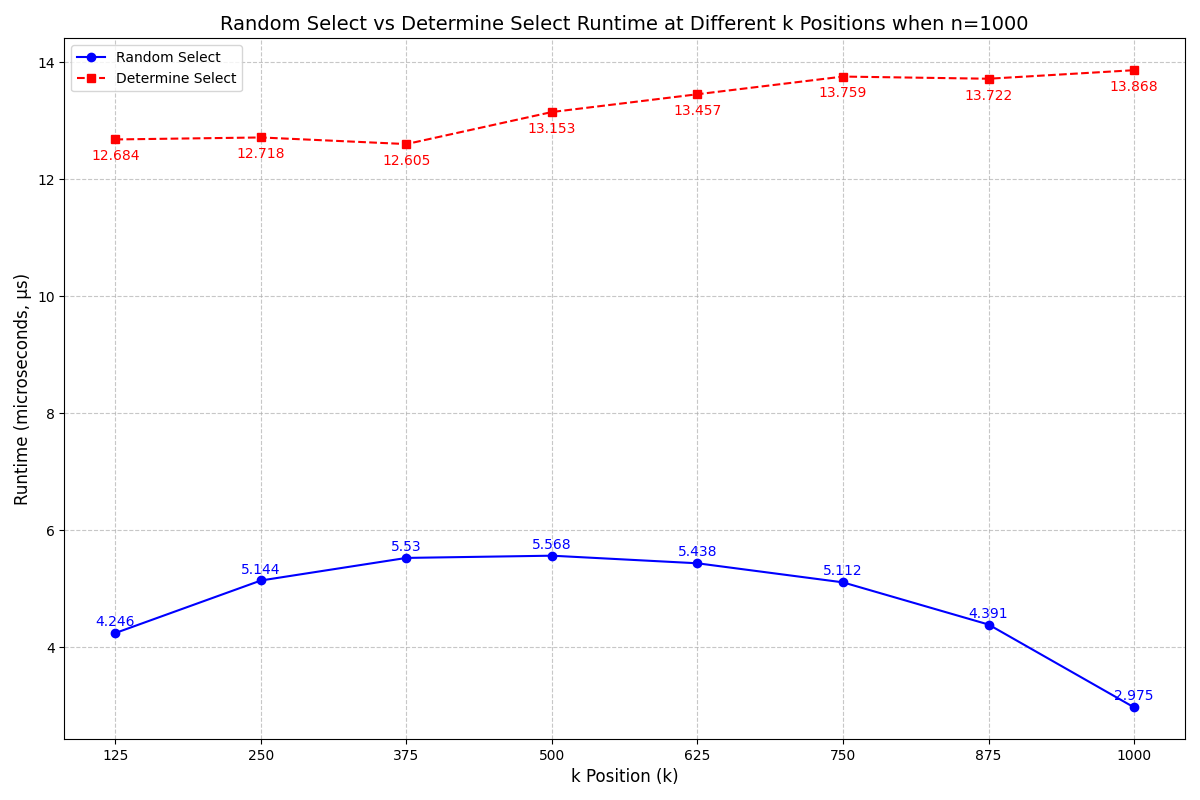
\includegraphics[width=0.7\textwidth]{../figure/1000.png}
    \caption{数组大小为 1000 时的运行时间比较}
\end{figure}
\begin{figure}[H]
    \centering
    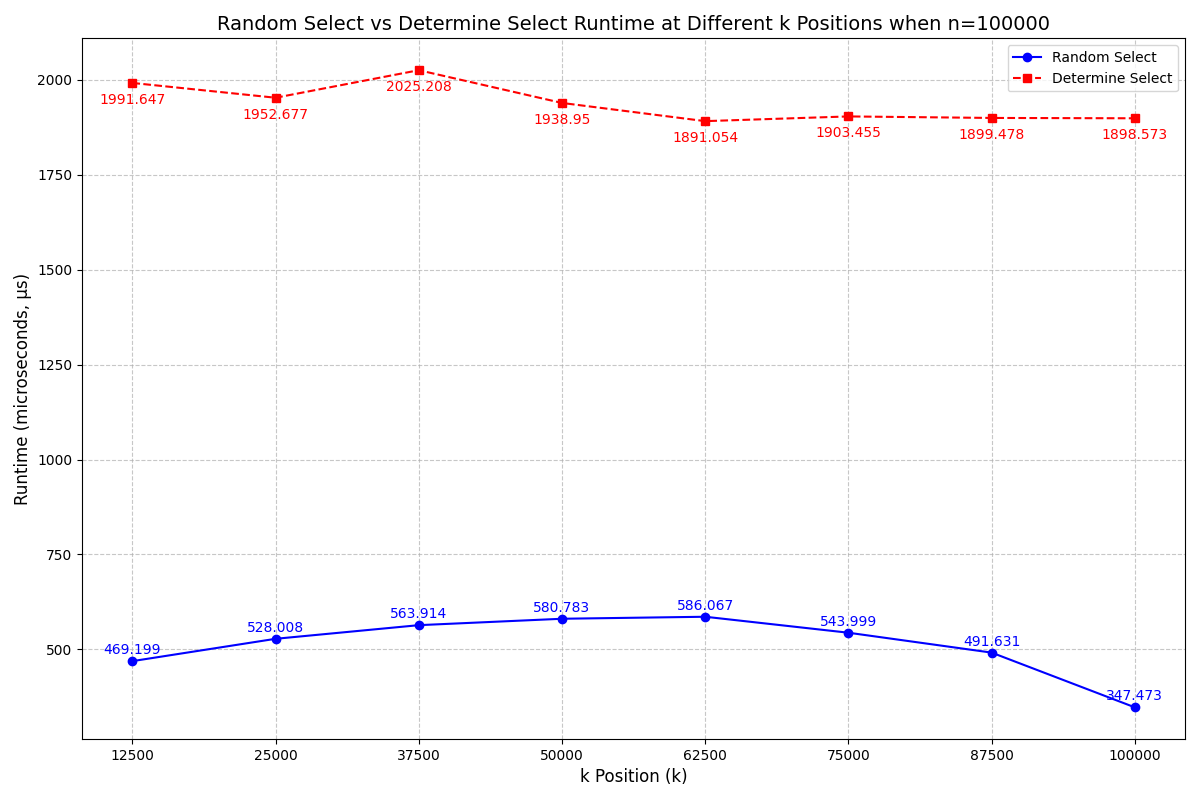
\includegraphics[width=0.7\textwidth]{../figure/100000.png}
    \caption{数组大小为 100000 时的运行时间比较}
\end{figure}
\begin{figure}[H]
    \centering
    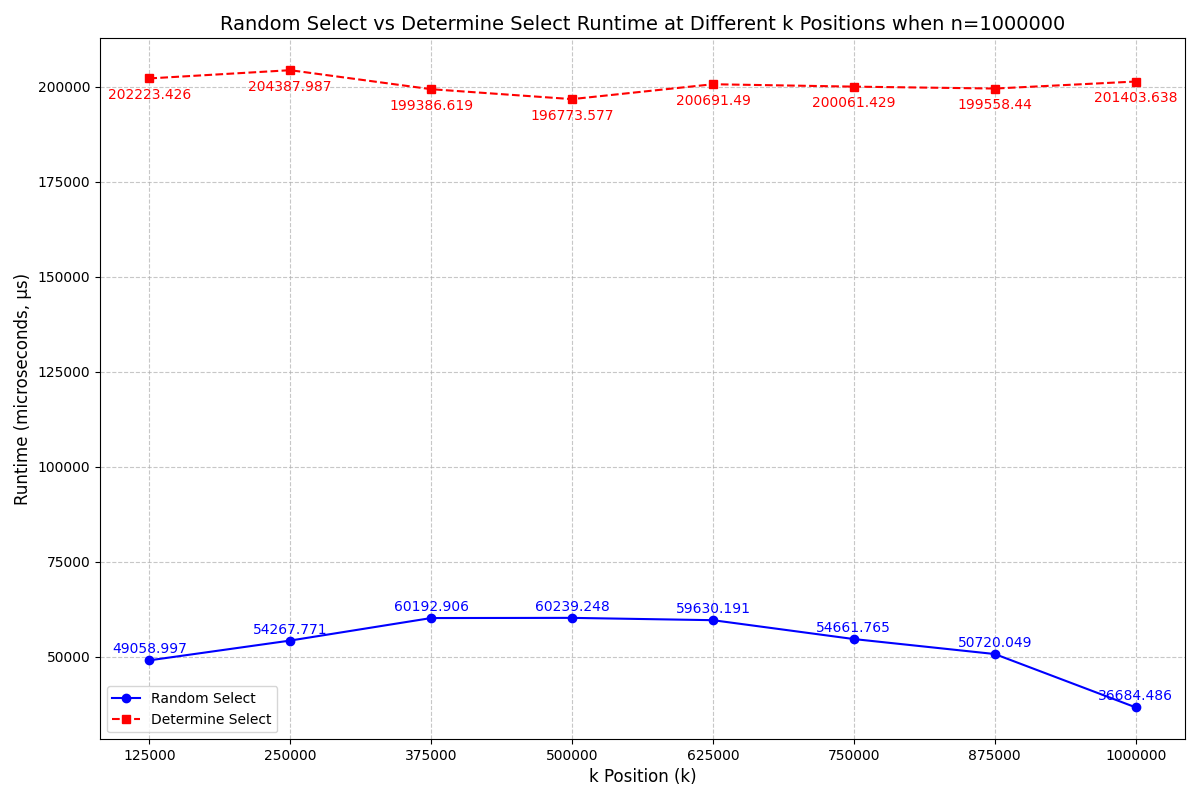
\includegraphics[width=0.7\textwidth]{../figure/1000000.png}
    \caption{数组大小为 1000000 时的运行时间比较}
\end{figure}
\begin{figure}[H]
    \centering
    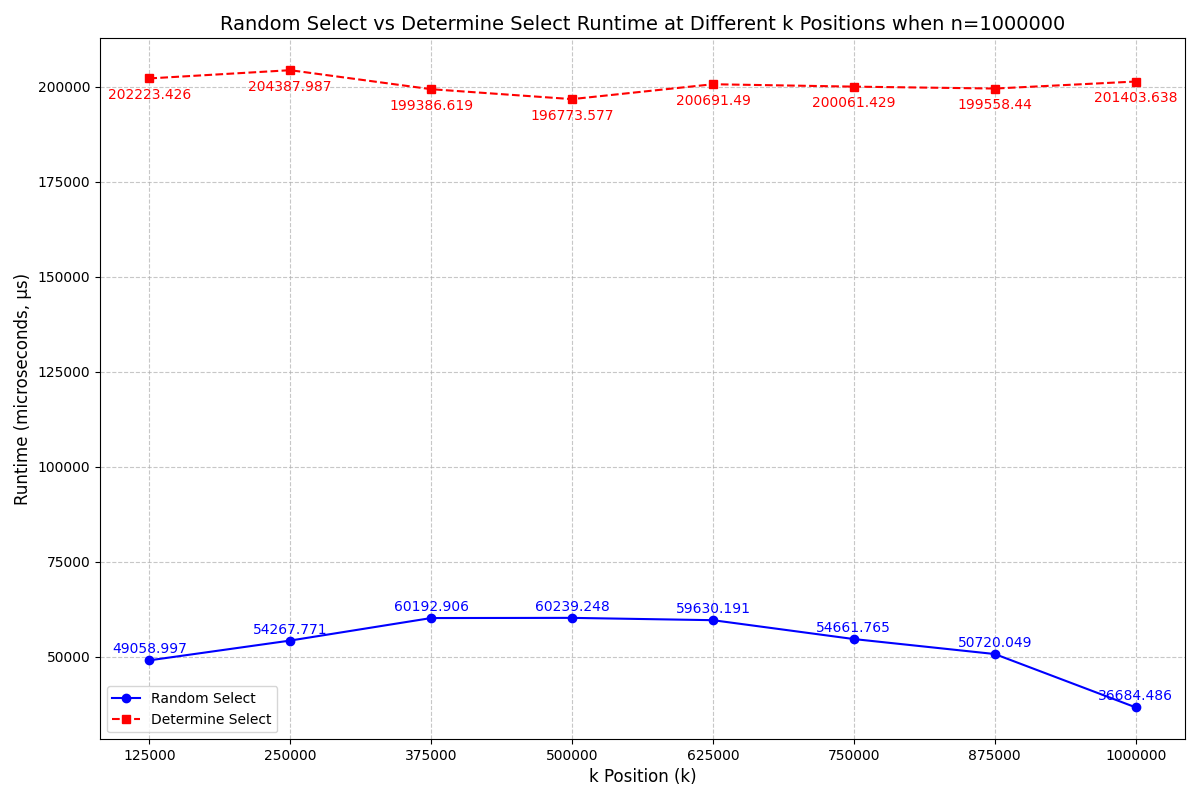
\includegraphics[width=0.7\textwidth]{../figure/10000000.png}
    \caption{数组大小为 10000000 时的运行时间比较}
\end{figure}

可以看到,在 $k$ 依次取在有序后的头部、中间和尾部时,随机选择方法呈现出运行时间先增加后减少的趋势,而确定性选择方法则保持线性稳定上下波动的运行时间。且确定性选择方法的时间一直保持在随机选择方法的 3-4 倍左右。

\subsection{分析特点比较}
确定性选择算法通过确保每次分区都能有效地缩小搜索范围,保持了线性稳定的运行时间,不受 $k$ 取值位置的影响。而随机选择方法由于枢轴选择的随机性,在 $k$ 取值靠近数组的头部或尾部时,可能导致较深的递归调用,从而使运行时间增加;当  k  取值靠近中间时,分割更为均匀,递归深度较浅,运行时间相应减少。因此,QuickSelect 在不同  k  值下呈现出运行时间先增加后减少的趋势,而确定性选择方法则保持了线性稳定的运行时间。
\begin{itemize}
    \item \textbf{算法常数因子的影响}:确定性选择算法通常将数组分成固定大小(如5)的组,并对每组进行排序以找到中位数。这一过程涉及大量的交换和比较操作,尤其是在处理大规模数据时,分组和排序的开销显著。在确定性选择算法中,需要递归地在中位数数组中寻找中位数的中位数,这进一步增加了递归调用的开销。而随机化选择只需选择一个随机枢轴,并进行一次简单的分区操作。相比于确定性选择算法,随机化选择的分区过程更为直接和高效,涉及的操作更少。
    \item \textbf{缓存友好性和内存访问模式}:确定性选择算法在分组和排序过程中,会频繁地跳跃访问数组元素,这种不连续的内存访问模式会导致缓存未命中率增加,从而降低性能。随机化选择的分区操作通常在数组中进行顺序扫描和交换,这种连续的内存访问模式更符合现代处理器的缓存机制,能够更好地利用缓存,提升运行效率。
    \item \textbf{算法实现的复杂性}:确定性选择算法涉及分组、排序、递归选择中位数等多个步骤,代码实现较为复杂,容易引入额外的开销。随机化选择的实现相对简单,主要包括选择随机枢轴和进行分区操作,代码简洁高效,减少了不必要的开销。
    \item \textbf{实际数据分布的影响}:无论数据如何分布,确定性选择算法都能保证线性时间复杂度。
\end{itemize}
因此,在实际应用中,尤其是对于大多数数据分布情况,随机化选择算法由于其较低的常数因子、更好的缓存友好性和更简洁的实现,通常表现得更快,尽管它在最坏情况下可能退化为 $O(n)$ 的时间复杂度。不过,最坏情况发生的概率极低,尤其是在随机化策略有效的情况下,使得随机化选择成为实际中更为常用和高效的选择算法。

\subsection{执行多次查找后运行的变化}

\subsubsection{随机选择}

首先对随机选择进行了测试,选取数组大小为 1000000 的不同 $k$ 取值进行测试,每个 $k$ 执行 10000 次,结果如~\autoref{fig:random_continue} 所示。\begin{figure}[htbp]
    \centering
    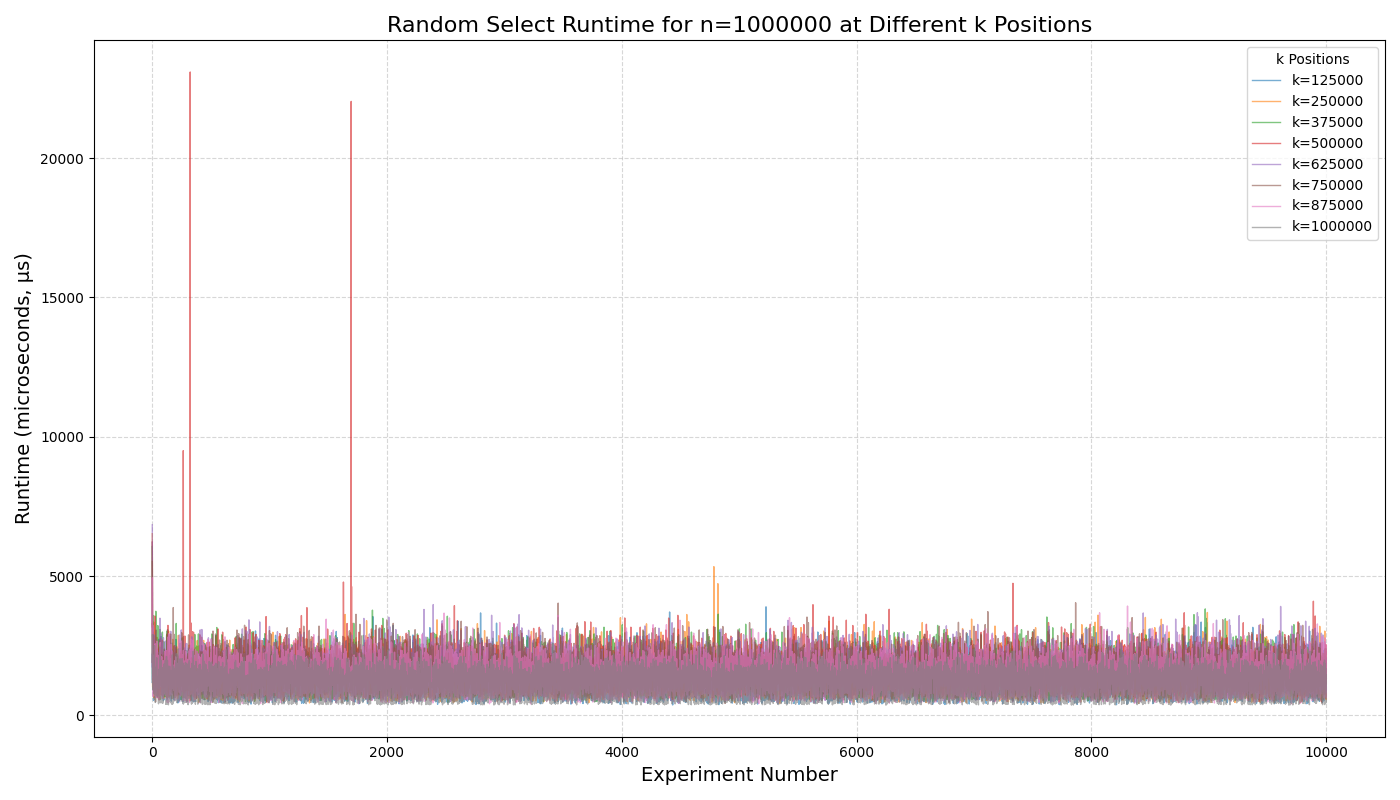
\includegraphics[width=0.7\textwidth]{../figure/random_continue.png}
    \caption{随机选择连续执行 10000 次查找运行时间}
    \label{fig:random_continue}
\end{figure}

可以看到,执行多次查找后,随机选择方法的运行时间并没有明显降低。依然是处于明显波动的状态。原因在于随机选择通选择枢轴是随机的,这种随机性使得即使数组部分有序,枢轴选择仍然可能导致不平衡的划分。其次,数组的部分有序性可能不足以显著减少比较和交换操作的数量,因为随机选择的核心操作仍然需要遍历整个数组并进行划分,即使某些区域已经有序,这些局部有序性对全局操作的优化效果有限。

此外可以看到图中存在明显高于其他值的特异值,这反映了随机选择的缺点,即在最坏情况下时间复杂度可能到达 $O(n^2)$,尽管发生的概率极低,在 10000 次重复实验中还是会发生。

考虑到异常值可能会影响大部分数值情况下的规律判断,选择用四分位数距离($IQR$)利用数据的第25百分位数($Q_1$)和第75百分位数($Q_3$),定义异常值为低于$Q_1 - 1.5 * IQR$或高于$Q_3 + 1.5 * IQR$的值对数据进行了清洗,该方法对数据的分布不做假设,相较于其他方法如 Z-Score 更加稳健。清洗后的时间变化如~\autoref{fig:random_continue_clean}。
\begin{figure}[htbp]
    \centering
    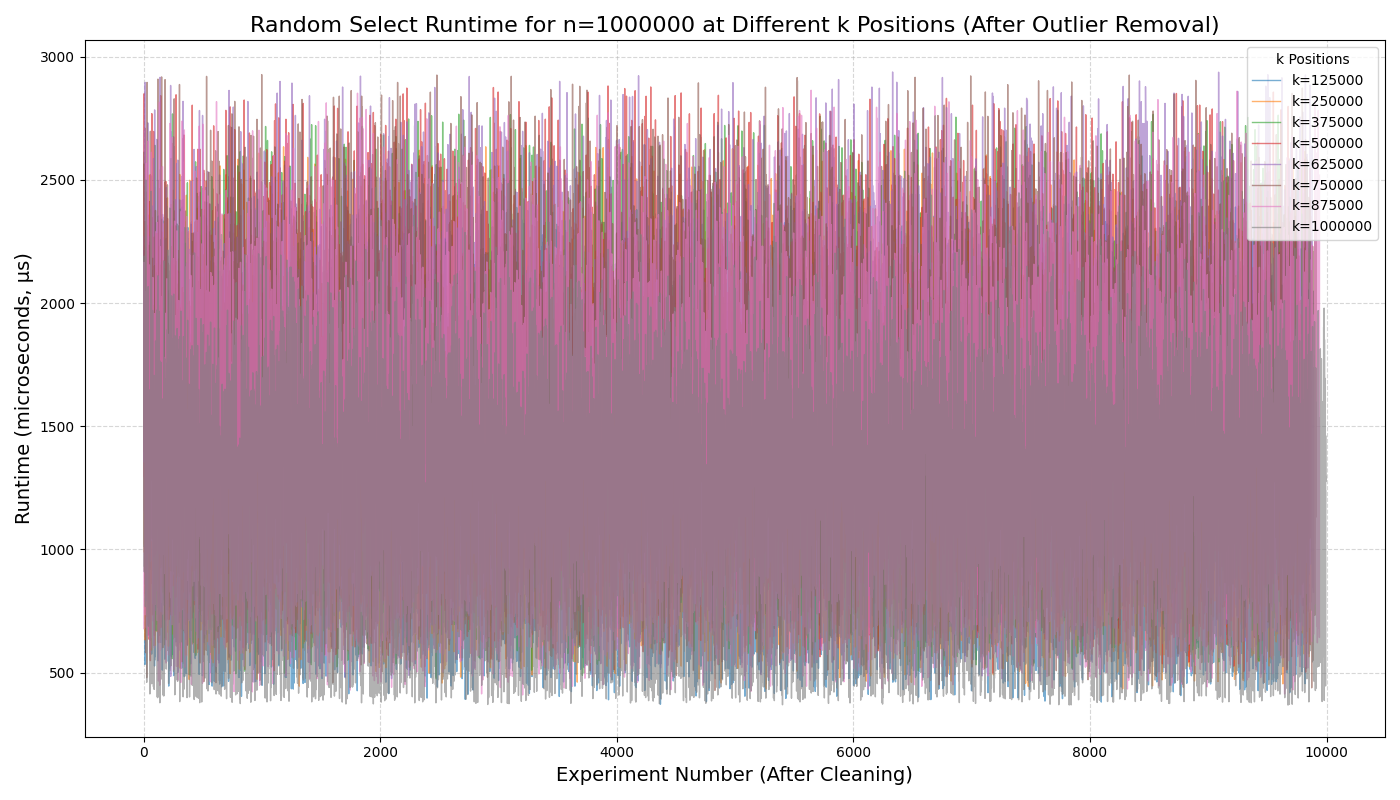
\includegraphics[width=0.7\textwidth]{../figure/random_continue_clean.png}
    \caption{清洗异常值后随机选择运行时间比较}
    \label{fig:random_continue_clean}
\end{figure}

可以看到,仍然没有明显的下降趋势。

\subsubsection{确定性选择}
随后对确定性选择进行了测试。实验次配置保持不变,实验结果如~\autoref{fig:determine_continue} 所示。\begin{figure}
    \centering
    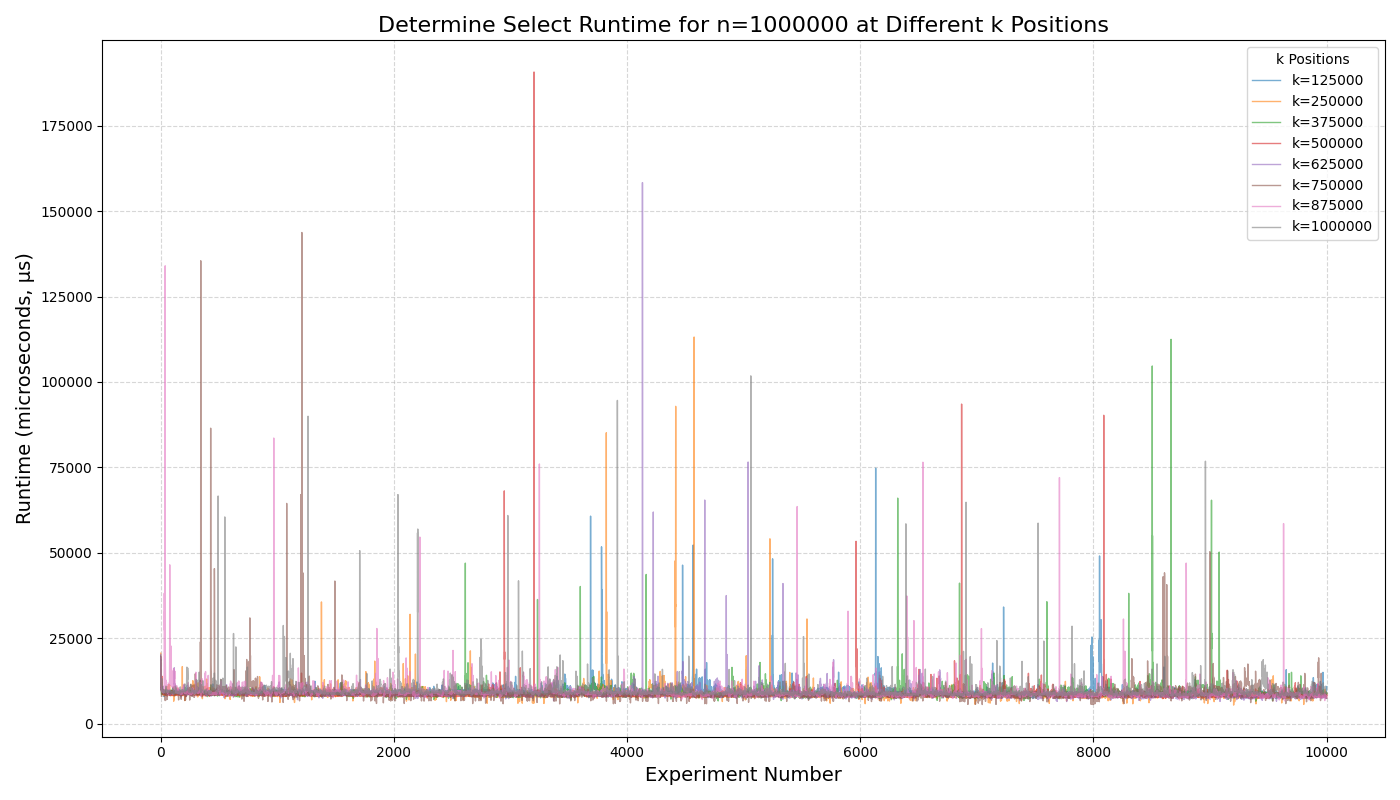
\includegraphics[width=0.7\textwidth]{../figure/determine_continue.png}
    \caption{确定性选择连续执行 10000 次查找运行时间}
    \label{fig:determine_continue}
\end{figure}

可以看到仍然存在特异值,但与随机选择相比,确定性选择的特异值相差没那么大,而且可能会收到实验环境的影响。采用相同的方法去掉特异值后如~\autoref{fig:determine_continue_clean} 所示:
\begin{figure}[htbp]
    \centering
    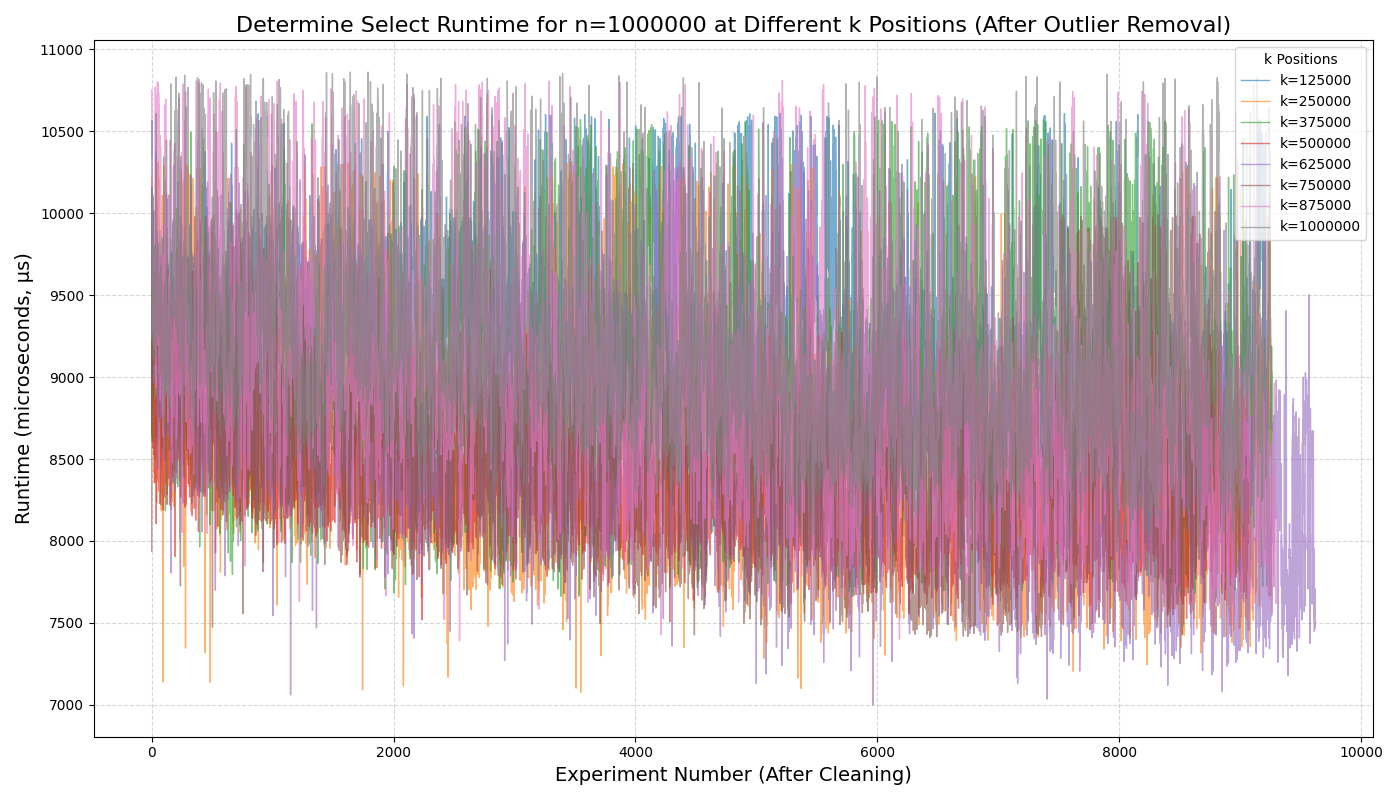
\includegraphics[width=0.7\textwidth]{../figure/determine_continue_clean.png}
    \caption{清洗异常值后确定性选择运行时间比较}
    \label{fig:determine_continue_clean}
\end{figure}

可以看到随着反复查找次数的增加,确定性选择的时间存在着波动中降低的趋势。但是通过分析可以知道,我们使用``中位数的中位数''方法选择枢轴,即使数据是有序的,算法仍会分组并计算每组的中位数,再从这些中位数中递归找到``中位数的中位数''作为枢轴,即算法不依赖数据本身的有序性,因此,数据的初始有序性不会显著影响这一过程的时间复杂度和流程。

但是从结果分析,原因可能在于在有序数据中,分区操作变得更加顺滑,因为当数据接近有序时,划分区域时不需要大量的数据移动。现代计算机的缓存机制对访问连续内存块的数据优化较好,因此当数据接近有序时,分区时访问的内存位置更加一致,缓存命中率提升,导致执行时间减少。此外,数据的有序性会使得每次选择的枢轴 ``中位数的中位数'' 能够将数组近乎均匀地分割为两部分,即每次分割后,左右子数组的大小大致相等(接近 $n/2$),接近算法的最好情况。

此外,\texttt{findMedian} 函数中的排序操作(\texttt{std::sort})会受数据有序性的影响。对于完全有序的数据,排序可能更快。然而,这种排序仅用于小的子数组(每组最多5个元素),这对整体复杂度的影响非常有限。因此,对整体的效率有待考究。

\subsubsection{进一步探究}

为了探究有序数据是否会对确定性选择的运行时间产生影响,我们将之前产生的数组大小 $n$为 1000000 的随机数字排序成有序数据后,对 $k = n / 2$ 的确定性选择进行了对比测试,结果如~\autoref{fig:sorted} 所示。
\begin{figure}[htbp]
    \centering
    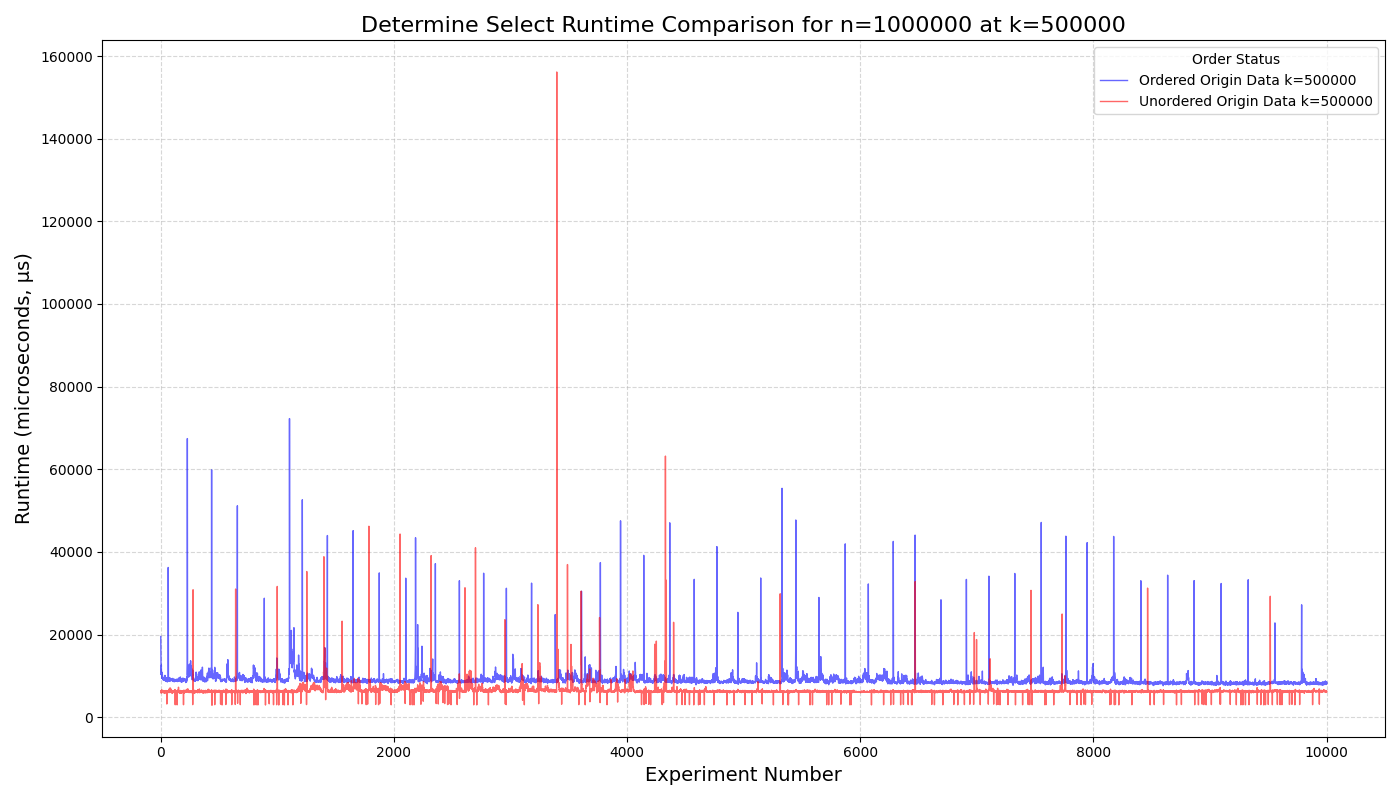
\includegraphics[width=0.7\textwidth]{../figure/determine_continue_order_vs_unorder.png}
    \caption{有序与无序数据的确定性选择运行时间对比}
    \label{fig:sorted}
\end{figure}

为了便于观察,数据清洗后的结果如~\autoref{fig:sorted_clean} 所示。
\begin{figure}[htbp]
    \centering
    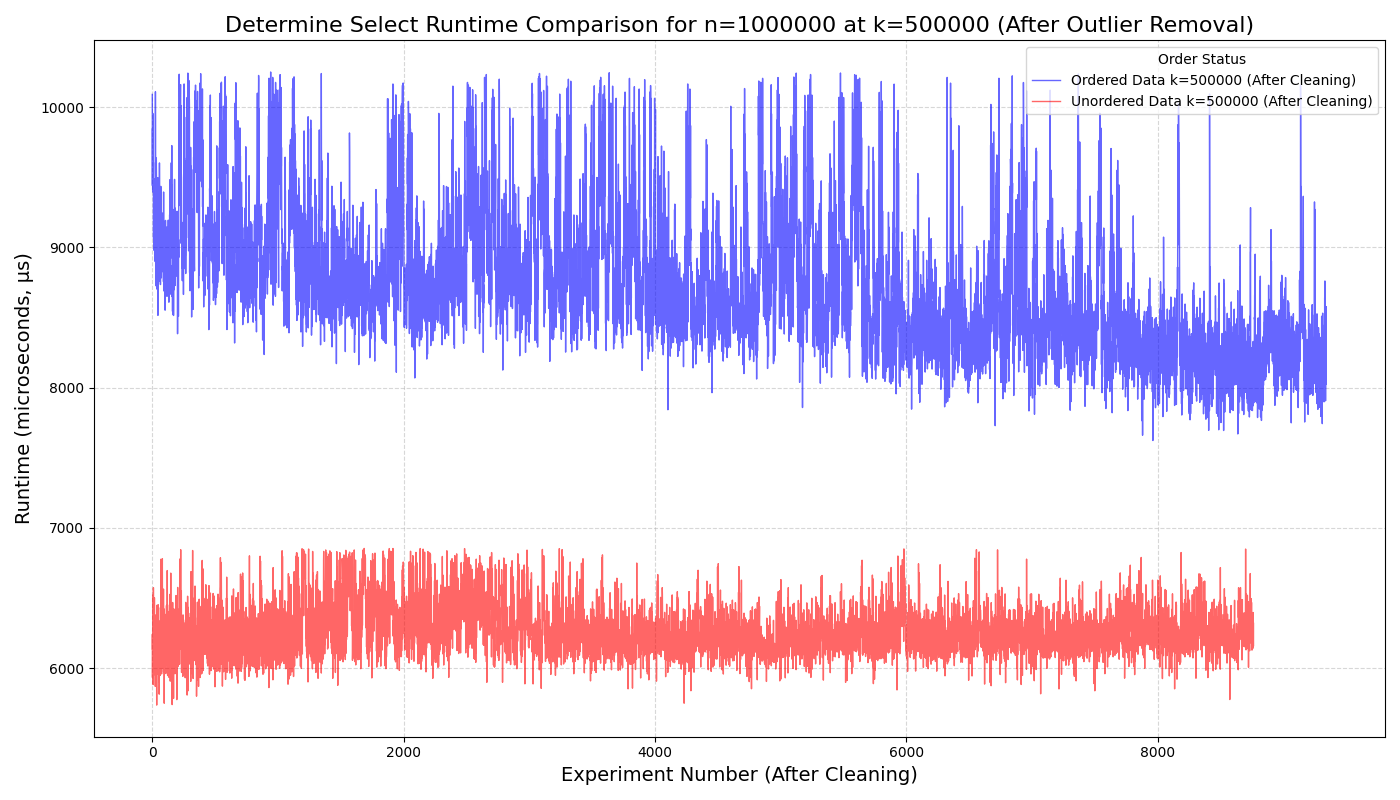
\includegraphics[width=0.7\textwidth]{../figure/determine_continue_order_vs_unorder_cleaned.png}
    \caption{清洗异常值后有序与无序数据的确定性选择运行时间对比}
    \label{fig:sorted_clean}
\end{figure}

可以直观看到,有序数据会对确定性选择的运行时间产生积极影响。有序数据的确定性选择运行时间明显低于无序数据,且有序数据的运行时间更加稳定,波动较小。更加验证了我们的猜想。
\section{算法改进}

\subsection{对确定性选择方法的改进}

由于实验结果表明,确定性选择方法的时间复杂度常数项较大,性能还值得改进。在实际应用中,我们可以考虑以下几种改进方法来减少常数大小:\begin{itemize}
    \item \textbf{减少 \texttt{findMedian} 中的排序开销}:目前的 \texttt{findMedian} 函数对每组的元素进行完全排序,这在最坏情况下是 $O(5 \log 5)$ ,尽管5是常数。实际上,我们只需要找到中位数,而不必对整个数组排序,可以使用选择算法来找出中位数,而不是完全排序。
    \item \textbf{减少对枢轴元素的查找开销}:目前代码通过 \texttt{std::find} 查找 \texttt{medianOfMedians} 的位置,这是线性时间操作。在分区操作中,可以结合分区和查找来减少一次遍历。通过使用 \texttt{partitionAroundPivot} 在分区的过程中查找并移动枢轴,避免二次遍历。
    \item \textbf{递归优化}:通过循环替代递归,减少递归深度,从而提升性能。
\end{itemize}

其算法的逻辑还是与之前类似,我们在数据量 $n$ 为 1000000 的情况下进行了测试,结果如~\autoref{fig:improve} 所示。为了保证不受系统等其他因素的干扰,我们没有采用之前改进前的测试数据,而是同时再次进行测试。
\begin{figure}[htbp]
    \centering
    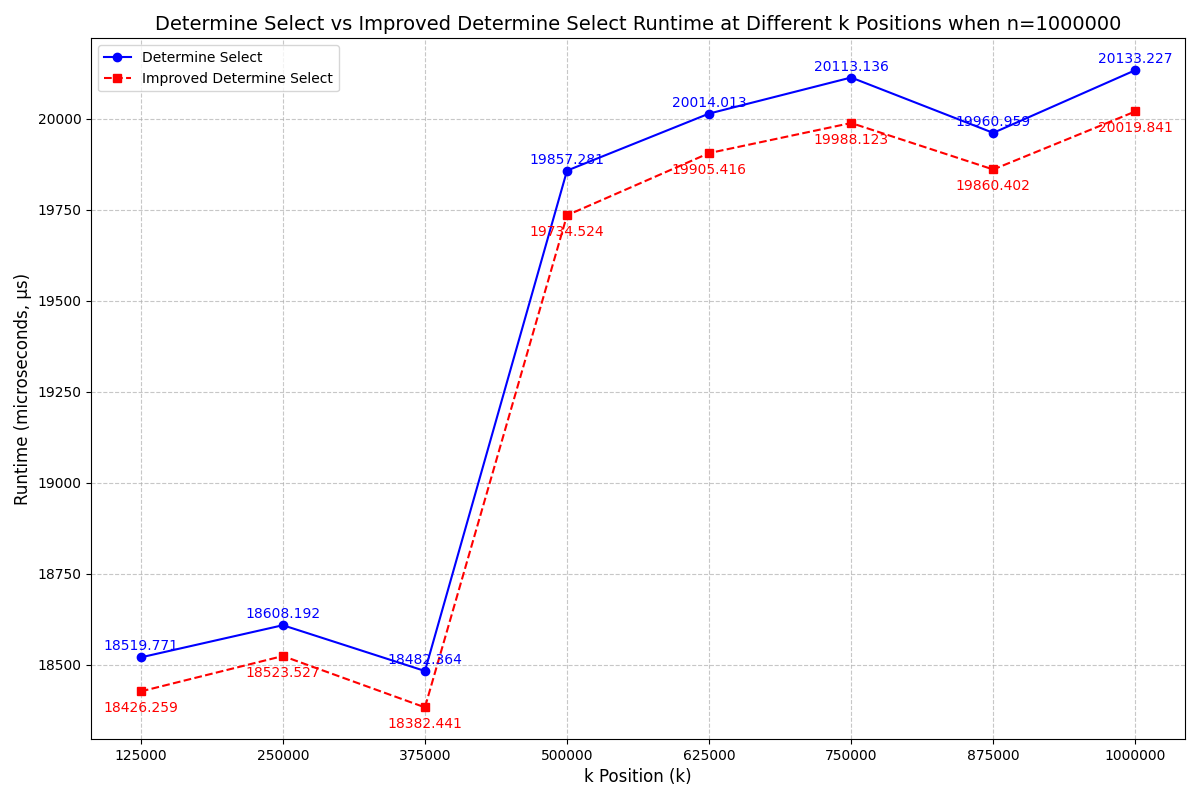
\includegraphics[width=0.7\textwidth]{../figure/determine_compare_1000000.png}
    \caption{改进前后的确定性选择运行时间对比}
    \label{fig:improve}
\end{figure}

可以发现提升了约 120 us。这说明我们的改进方法是有效的,可以减少确定性选择方法的常数项开销,提升算法性能。

\subsection{未完成的探究}

对于确定性时间分组大小的选择,在实验中,我们选择了分组大小为 5,这是一个经验值。在实际应用中,分组大小的选择可能会影响算法的性能。较小的分组大小可能会导致更多的分组和排序操作,增加额外开销;较大的分组大小可能会导致中位数的估计不准确,影响枢轴的选择。因此,如何选择合适的分组大小是一个值得研究的问题。

此外,数据有序性对确定性选择的运行时间影响也可能与分组大小有关。二者之间的关系也值得深入探究。但是由于时间关系,上述研究没有完成。

\section{总结}

这个实验让我对分治算法有了更深的理解,特别是在选择第 $k$ 大元素的场景下。通过设计和比较随机选择和确定性选择的方法,我体会到了算法效率、理论保证和实际应用之间的微妙平衡。

虽然确定性选择算法通过中位数的中位数策略确保了最坏情况下的线性时间复杂度,但实验中也暴露了其操作复杂度高、常数因子较大的问题。虽然理论上的保证看起来很理想,但在实际中往往需要牺牲简单性和实用性。相比之下,随机选择算法虽然最坏情况下的复杂度可能是二次的,但在实际应用中,尤其是对于典型的数据分布,其表现通常非常好。这让我明白了一个关键的道理:实际效率往往比最坏情况的理论保证更重要,特别是当随机化方法可以有效避免极端情况时。

另一个重要的收获是数据特性对算法性能的影响。当数据有序或无序时,两种方法的表现会有所不同,这让我感到很有趣,并对其展开了深入研究。尤其是在有序数据上,确定性方法的性能有所提升,这表明即使是确定性算法,也可以从输入数据的特性中获益,这和我最初认为其性能不受输入顺序影响的预期有些不同。

此外,这次实验让我更加认识到实现细节的重要性。像如何查找中位数、如何管理枢轴元素等小的实现选择,都会显著影响算法的性能。这让我更加明白,算法设计不仅是选择什么算法,更重要的是如何去实现它,这直接影响它的效果。

总的来说,这次实验让我意识到,从理论到实践的过程是复杂且充满权衡的。它加深了我对算法思想在面对真实数据和性能限制时如何演变的理解。这次练习在数学严谨性与实践适应性之间找到了平衡,也让我在未来的工作中对算法选择有了更多思考和信心。

\appendix

\section{关键源码}

\subsection{随机选择算法}

\begin{cppcode}
// 快速选择算法:查找第 k 大的元素(k 从 1 开始)
int quickSelect(std::vector<int>& nums, int left, int right, int k, std::mt19937& gen) // NOLINT
{
    if (left == right) {
        return nums[left];
    }

    // 随机选择枢轴
    std::uniform_int_distribution<> dis(left, right);
    int pivotIndex = dis(gen);
    int pivot = nums[pivotIndex];

    // 移动枢轴到末尾
    std::swap(nums[pivotIndex], nums[right]);

    // 分区
    int storeIndex = left;
    for (int i = left; i < right; ++i) {
        if (nums[i] > pivot) { // 查找第 k 大,因此使用 > 符号
            std::swap(nums[i], nums[storeIndex]);
            storeIndex++;
        }
    }
    // 将枢轴放到正确的位置
    std::swap(nums[storeIndex], nums[right]);

    // 计算枢轴位置相对于第 k 大的位置
    int count = storeIndex - left + 1;
    if (count == k) {
        return nums[storeIndex];
    }
    if (k < count) {
        return quickSelect(nums, left, storeIndex - 1, k, gen);
    }
    return quickSelect(nums, storeIndex + 1, right, k - count, gen);
}
\end{cppcode}

\subsection{确定性选择算法}
\begin{cppcode}
// 辅助函数:找到数组的中位数
int findMedian(std::vector<int>& nums, int left, int right) {
    std::sort(nums.begin() + left, nums.begin() + right + 1);
    return nums[left + (right - left) / 2];
}
// 中位数中位数算法:确定性的线性时间选择算法
int deterministicSelect(std::vector<int>& nums, int left, int right, int k) { //NOLINT
    // 如果数组足够小,直接返回中位数
    if (right - left + 1 <= groupSize) {
        return findMedian(nums, left, right);
    }

    // 将数组分成每组最多5个元素,找到每组的中位数
    std::vector<int> medians;
    for (int i = left; i <= right; i += groupSize) {
        int sub_right = std::min(i + 4, right);
        medians.push_back(findMedian(nums, i, sub_right));
    }

    // 递归地找到中位数的中位数
    int medianOfMedians = deterministicSelect(medians, 0, static_cast<int>(medians.size()) - 1, static_cast<int>(medians.size()) / 2);

    // 找到中位数中位数的位置
    std::vector<int>::difference_type pivotIndex = std::distance(nums.begin(), std::find(nums.begin() + left, nums.begin() + right + 1, medianOfMedians));

    // 移动枢轴到末尾
    std::swap(nums[pivotIndex], nums[right]);

    // 分区
    int storeIndex = left;
    for (int i = left; i < right; ++i) {
        if (nums[i] > medianOfMedians) { // 查找第 k 大,因此使用 > 符号
            std::swap(nums[i], nums[storeIndex]);
            storeIndex++;
        }
    }
    // 将枢轴放到正确的位置
    std::swap(nums[storeIndex], nums[right]);

    // 计算枢轴位置相对于第 k 大的位置
    int count = storeIndex - left + 1;
    if (count == k) {
        return nums[storeIndex];
    }
    if (k < count) {
        return deterministicSelect(nums, left, storeIndex - 1, k);
    }
    return deterministicSelect(nums, storeIndex + 1, right, k - count);
}
\end{cppcode}

\subsection{改进后的确定性选择算法}
\begin{cppcode}
// 辅助函数:找到数组的中位数
int findMedian(std::vector<int>& nums, int left, int right) {
    std::sort(nums.begin() + left, nums.begin() + right + 1);
    return nums[left + (right - left) / 2];
}

// 中位数中位数算法:确定性的线性时间选择算法
int deterministicSelect(std::vector<int>& nums, int left, int right, int k) { //NOLINT
    // 如果数组足够小,直接返回中位数
    if (right - left + 1 <= groupSize) {
        return findMedian(nums, left, right);
    }

    // 将数组分成每组最多5个元素,找到每组的中位数
    std::vector<int> medians;
    for (int i = left; i <= right; i += groupSize) {
        int sub_right = std::min(i + 4, right);
        medians.push_back(findMedian(nums, i, sub_right));
    }

    // 递归地找到中位数的中位数
    int medianOfMedians = deterministicSelect(medians, 0, static_cast<int>(medians.size()) - 1, static_cast<int>(medians.size()) / 2);

    // 找到中位数中位数的位置
    std::vector<int>::difference_type pivotIndex = std::distance(nums.begin(), std::find(nums.begin() + left, nums.begin() + right + 1, medianOfMedians));

    // 移动枢轴到末尾
    std::swap(nums[pivotIndex], nums[right]);

    // 分区
    int storeIndex = left;
    for (int i = left; i < right; ++i) {
        if (nums[i] > medianOfMedians) { // 查找第 k 大,因此使用 > 符号
            std::swap(nums[i], nums[storeIndex]);
            storeIndex++;
        }
    }
    // 将枢轴放到正确的位置
    std::swap(nums[storeIndex], nums[right]);

    // 计算枢轴位置相对于第 k 大的位置
    int count = storeIndex - left + 1;
    if (count == k) {
        return nums[storeIndex];
    }
    if (k < count) {
        return deterministicSelect(nums, left, storeIndex - 1, k);
    }
    return deterministicSelect(nums, storeIndex + 1, right, k - count);
}
\end{cppcode}
\end{document}
